\chapter[DIFUSÃO DE CALOR 2D EM REGIME PERMANENTE]{DIFUSÃO DE CALOR 2D EM REGIME PERMANENTE}

Para o estudo da difusão de calor 2D em regime permanente, parte-se das seguintes hipóteses:
\begin{itemize}
    \item Difusão de calor 2D
    \item Regime permanente
    \item Propriedades termofísicas constantes
    \item Presença de termo fonte
\end{itemize}

Sob esses hipóteses, tem-se a seguinte equação governante:

\begin{equation}
    \label{eq:8.1}
    \frac{\partial^2 T}{\partial x^2} + \frac{\partial^2 T}{\partial y^2} = S^\phi
\end{equation}

Que pode ser reescrita como:

\begin{equation}
    \label{eq:8.2}
    \vec{\nabla} \cdot (\vec{\nabla} T) = S^\phi
\end{equation}

Tal expressão deve ser, então, integrada para cada volume de controle do domínio discretizado, de modo que:

\begin{equation}
    \label{eq:8.3}
    \int_{vc} \vec{\nabla} \cdot (\vec{\nabla}T) dv = \int_{vc}S^\phi dv
\end{equation}

Aplicando-se, na sequência, o teorema da divergência de Gauss no lado esquerdo da equação anterior, tem-se:

\begin{equation}
    \label{eq:8.4}
    \int_A \hat{n} \cdot (\vec{\nabla T}) dA = \int_{vc} S^\phi dv
\end{equation}

Ou seja,

\begin{equation}
    \label{eq:8.5}
    \sum_{superficies} \int_{\nabla A_i} \hat{n} \cdot (\vec{\Delta}T)dA = \int_{vc} S^\phi dv
\end{equation}

A integração de superfície de cada elemento é aproximada pelo produto interno entre o vetor normal (direcionado para fora do volume de controle) à superfície $
hat{n_i}$ e um vetor de fluxo difusivo $(\vec{\Delta}T)$ que atravessa a superfície do elemento de controle $(\Delta A_i)$. O primeiro termo da equação \ref{eq:8.5} pode ser aproximado empregando-se o método de diferenças centrais ao longo da linha $PA$. Deste modo,

\begin{equation}
    \label{eq:8.6}
    \int_{\Delta A_i} \hat{n_i} \cdot (\vec{\nabla}T)dA \approx \hat{n_i} \cdot (\vec{\nabla}T) \Delta A_i \approx \frac{T_A - T_P}{\Delta \xi} \Delta A_i
\end{equation}

\begin{figure}[ht]
    \begin{subfigure}{.5\textwidth}
        \centering
        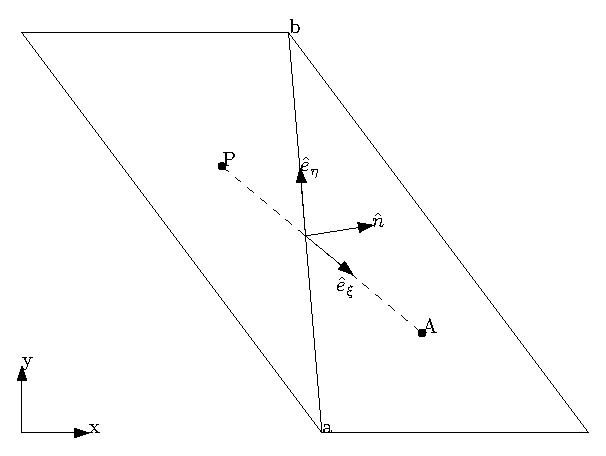
\includegraphics[width=.8\linewidth]{fig/difusao-cruzada-a.eps}
        \caption{}
        \label{fig:8.1-a}
    \end{subfigure}
    \begin{subfigure}{.5\textwidth}
        \centering
        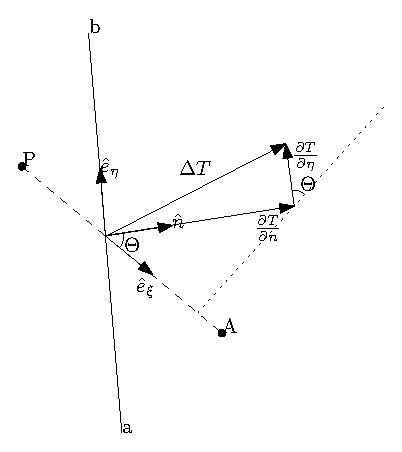
\includegraphics[width=.8\linewidth]{fig/difusao-cruzada-b.eps}
        \caption{}
        \label{fig:8.1-b}
    \end{subfigure}

    \begin{subfigure}{.5\textwidth}
        \centering
        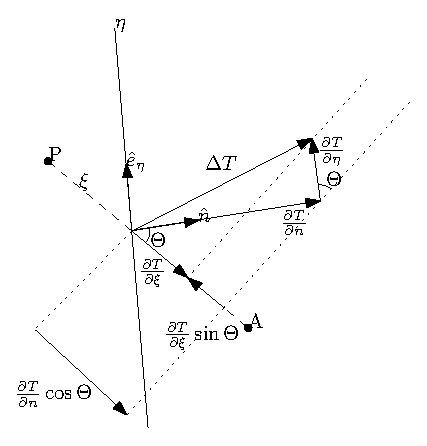
\includegraphics[width=.8\linewidth]{fig/difusao-cruzada-c.eps}
        \caption{}
        \label{fig:8.1-c}
    \end{subfigure}

    \caption{Esquemas para definição do termo de difusão cruzada}
    \label{fig:8.1}
\end{figure}

Na equação \ref{eq:8.6} $\Delta \xi$ é a distância entre os centroides A e P. Nota-se que a diferença central na equação \ref{eq:8.6} só é acurada se a linha que une os pontos A e P e o vetor normal unitário $\hat{n_i}$ estão na mesma direção, ou seja, a aproximação só é correta no caso em que a malha é completamente ortogonal. Normalmente, em malhas não-estruturadas as linhas que conectam os centroides P e A não são paralelas ao vetor normal unitário $\hat{n_i}$. Isto é conhecido como não-ortogonalidade de malha (mesh skewness ou mesh non-orthogonality). O cálculo do fluxo na equação \ref{eq:8.6} deve, desse modo, ser corrigido pela adição de uma contribuição provocada pela não-ortogonalidade. Existem diversos meios de realizar essa correção, mas a forma mais comum é a de introduzir um termo conhecido como difusão cruzada (cross diffusion), que é tratada como termo-fonte na equação discretizada.

Seguindo-se a metodologia proposta por Mathur e Murthy (1997), tem-se que ao termo de difusão cruzada é obtido, introduzindo-se as coordenadas $\xi$ e $\eta$, sendo: $\xi$ definida ao longo da linha que une os pontos A e P, e $\eta$ ao longo da face do volume de controle (ao longo da linha que une os vértices a e b). Desse modo, o gradiente $\vec{\Delta}T$ pode ser expresso por:

\begin{equation}
    \label{eq:8.7}
    \vec{\nabla}T = \frac{\partial T}{\partial x}\hat{i} + \frac{\partial T}{\partial y}\hat{j} = \frac{\partial T}{\partial n}\hat{n} + \frac{\partial T}{\partial \eta}\hat{e_\eta}
\end{equation}

Sendo $\hat{i}$ e $\hat{j}$ vetores unitários nas direções $x$ e $y$ e $\hat{n}$ e $\hat{e_\eta}$ vetores unitários ao longo das direções normal e tangencial.

O vetor unitário normal $\hat{n}$, bem como os vetores unitários nas direções $\xi$ e $\eta$, $\hat{e_\xi}$ e $\hat{e_\eta}$, respectivamente, podem ser expressas através das seguintes relações envolvendo centroides e vértices:

\begin{equation}
    \label{eq:8.8}
    \hat{n} = \frac{\Delta y}{\Delta A_i}\hat{i} - \frac{\Delta x}{\Delta A_i}\hat{j} = \frac{y_b - y_a}{\Delta \eta}\hat{i} - \frac{x_b - x_a}{\Delta \eta}\hat{j}
\end{equation}

\begin{equation}
    \label{eq:8.9}
    \hat{e_\xi} = \frac{x_A - x_P}{\Delta \xi}\hat{i} + \frac{y_A - y_P}{\Delta \xi}\hat{j}
\end{equation}

\begin{equation}
    \label{eq:8.10}
    \hat{e_\eta} = \frac{x_b - x_a}{\Delta \eta}\hat{i} + \frac{y_b - y_a}{\Delta \eta}\hat{j}
\end{equation}

Uma observação que deve ser feita a respeito da equação \ref{eq:8.6} é a que ela é uma aproximação real de $\partial T/\partial \xi$ apenas no caso de uma malha ortogonal, ou seja, quando $\partial T/\partial \xi = \partial T/\partial n$. Caso contrário, para malhas não-ortogonais, $\partial T/\partial \xi$ pode ser muito diferente de $\partial T/\partial n$.

Observa-se nas figuras \ref{fig:8.1-b} e \ref{fig:8.1-c} que $\partial T/\partial \xi$ corresponde ao comprimento da projeção do vetor $\vec{\Delta}T$ na direção de $\xi$. Empregando a equação \ref{eq:8.7}, pode-se representar também $\vec{\Delta}T$ como a soma de $(\partial T/\partial n)\hat{n}$ e $(\partial T/\partial \eta)\hat{e_\eta}$, conforme a figura \ref{fig:8.1-c}.

Para se obter uma melhor estimativa do fluxo normal $\hat{n} \cdot \vec{\Delta}T = \partial T/\partial n$, examina-se a relação entre a projeção de $\vec{\Delta}T$ na direção $\xi$ que é $(\partial T/\partial \xi)$ e as projeções nessa direção de duas componentes de $\vec{\Delta}T$ que são: $(\partial T/\partial n)\hat{n} \cdot \hat{e_\xi}$ e $(\partial T/\partial \eta)\hat{e_\eta} \cdot \hat{e_\xi}$.

Denotando-se o ângulo entre as direções $\hat{n}$ e $\xi$ por $\Theta$, tem-se que:

\begin{equation}
    \label{eq:8.11}
    \frac{\partial T}{\partial n} \hat{n} \cdot \hat{e_\xi} = \frac{\partial T}{\partial n} \cos{\Theta}
\end{equation}

e

\begin{equation}
    \label{eq:8.12}
    \frac{\partial T}{\partial \eta} \hat{e_\eta} \cdot \hat{e_\xi} = - \frac{\partial T}{\partial \eta} \sin{\Theta}
\end{equation}

Deste modo, tem-se que:

\begin{equation}
    \label{eq:8.13}
    \frac{\partial T}{\partial \xi} = \frac{\partial T}{\partial n}\cos{\Theta} - \frac{\partial T}{\partial \eta} \sin{\Theta}
\end{equation}

Recorda-se, então, que $\hat{n} \cdot \vec{\Delta}T = \partial T/\partial n$ e, rearranjando os termos da equação \ref{eq:8.13}, obtém-se o fluxo difusivo da equação \ref{eq:8.6}:

\begin{equation}
    \label{eq:8.14}
    \hat{n} \cdot \vec{\Delta}T = \frac{\partial T}{\partial n} = \frac{\partial T}{\partial \xi} \frac{1}{\cos{\Theta}} + \frac{\partial T}{\partial \eta} \tan{\Theta}
\end{equation}

Os dois gradientes que transportam T no lado direito da equação \ref{eq:8.14} podem ser aproximados por diferenças centrais (CDS):

\begin{equation}
    \label{eq:8.15}
    \frac{\partial T}{\partial \xi} = \frac{T_A - T_P}{\Delta \xi}
\end{equation}

\begin{equation}
    \label{eq:8.16}
    \frac{\partial T}{\partial \eta} = \frac{T_b - T_a}{\Delta \eta}
\end{equation}

Onde $\Delta \xi$ é a distância entre os centroides $A$ e $P_i$ e $\Delta \eta$ é a distância entre os vértices $a$ e $b$ ($\Delta \eta = \Delta A_i)$.

Na literatura, tem-se que $\partial T/\partial \xi$ e $\partial T/\partial \eta$ são chamaods de gradiente direto (Direct Gradient) e difusão cruzada (Cross Diffusion), respectivamente. A substituição das aproximações por diferenças centrais, equações \ref{eq:8.15} e \ref{eq:8.16} na equação \ref{eq:8.14} resulta em:

\begin{equation}
    \label{eq:8.17}
    \hat{n} \cdot \vec{\nabla}T \Delta A_i = \frac{\Delta A_i}{\cos{\Theta}} \frac{T_A - T_P}{\Delta \xi} + \Delta A_i \tan{\Theta} \frac{T_b - T_a}{\Delta \eta}
\end{equation}

Da figura \ref{fig:8.1}, observa-se que:

\begin{equation}
    \label{eq:8.18}
    \frac{1}{\cos \Theta} = \frac{1}{\hat{n}\cdot \hat{e_\xi}} = \frac{\hat{n} \cdot \hat{n}}{\hat{n} \cdot \hat{e_\xi}}
\end{equation}

e

\begin{equation}
    \label{eq:8.19}
    \tan{\Theta} = \frac{\sin{\Theta}}{\cos{\Theta}} = - \frac{\hat{e_\xi} \cdot \hat{e_\eta}}{\hat{n} \cdot \hat{e_\xi}}
\end{equation}

Lembrando-se que:

\begin{equation}
    \label{eq:8.20}
    \vec{a} \cdot \vec{b} = |a| |b| \cos{\Theta}
\end{equation}

e

\begin{equation}
    \label{eq:8.21}
    \cos{\pi / 2 = \alpha} = - \sin{\alpha}
\end{equation}

Deste modo, a equação \ref{eq:8.17} pode ser escrita na forma vetorial como:

\begin{equation}
    \label{eq:8.22}
    \hat{n} \cdot \vec{\nabla} T \Delta A_i = \frac{\hat{n} \cdot \hat{n} \Delta A_i}{\hat{n} \cdot \hat{e_\xi}} \frac{T_A - T_P}{\Delta \xi} - \frac{\hat{e_\xi} \cdot \hat{e_\eta} \Delta A_i}{\hat{n} \cdot \hat{e_\xi}} \frac{T_b - T_a}{\Delta \eta}
\end{equation}

Os fatores $\hat{n} \cdot \hat{n} \Delta A_i / (\hat{n} \cdot \hat{e_\xi})$ e $\hat{e_\xi} \cdot \hat{e_\eta} \Delta A_i / (\hat{n} \cdot \hat{e_\xi})$ podem ser obtidos da geometria dos elementos de malha.

Normalmente, o termo de disufão cruzada é tratado como termo-fonte na equação dicretizada. Deste modo, separando-se o termo de difusão cruzada da equação \ref{eq:8.22}, obtém-se:

\begin{equation}
    \label{eq:8.23}
    \hat{n} \cdot \vec{\nabla}T \Delta A_i = \frac{\hat{n} \cdot \hat{n} \Delta A_i}{\hat{n} \cdot \hat{e_\xi}} \frac{T_A - T_P}{\Delta \xi} + S_{DC}
\end{equation}

Para a estimativa do termo de difusão cruzada, é necessário avaliar o $\vec{\nabla}T$ ao longo da linha $ab$. Existem vários métodos que podem ser empregados nesse cáclulo. Um deles consiste em interpolar os valores de $T$ nodais (obtidas para os centroides) para calcular os valores de $T_a$ e $T_b$ e então estimar o gradiente. Empregando-se a média entre todos os pontos nodais vizinhos ao vértice $a$ conduz a:

\begin{equation}
    \label{eq:8.24}
    T_a = \frac{T_P + T_A + T_B + \dots}{N}
\end{equation}

Onde $N$ é o número total de nós (centroides) ao redor do vértice $a$. Uma alternativa é empregar uma média ponderada pela distância entre o vértice e os nós, cujo resultado é mais acurado, porém, também mais caro computacionalmente.

O termo-fonte, da equação \ref{eq:8.15}, é tratado de modo semelhante ao método empregado para malhas ortogonais, ou seja:

\begin{equation}
    \label{eq:8.25}
    \int_{vc} S^\phi dv = \bar{S} \Delta v
\end{equation}

Onde $\Delta v$ é o volume do volume de controle envolvido, e $\bar{S}$ é o valor médio de $S^\phi$ sobre todo o volume de controle.

A aproximação da equação \ref{eq:8.25}, com uma aproximação de segunda ordem de acurácia, é obtida ao se empregar o teorema do valor intermediário para integrais, substituindo-se o valor médio $\bar{S}$ pelo valor nodal da função $S$ aplicado no centroide do volume de controle. No caso bidimensional, o volume $\Delta v$ corresponde à área do elemento de malha multiplicada por um comprimento unitário na direção normal ao plano bidimensional. Assim:

\begin{equation}
    \label{eq:8.26}
    \int_{vc} S^\phi dv = S_P \Delta v
\end{equation}

No caso 2D tem-se que $\Delta v = \Delta A$.

Antes de efetuar o acoplamento das diversas partes da equação discretizada para se obter o sistema de equações lineares correspondente. A equação \ref{eq:8.23} será reescrita como:

\begin{equation}
    \label{8.27}
    \hat{n} \cdot \vec{\nabla}T \Delta A_i = D_i (T_A-T_P) + S_{DC,i}
\end{equation}

Onde

\begin{equation}
    \label{eq:8.28}
    D_i = \frac{\hat{n_i} \cdot \hat{n_i}}{\hat{n_i} \cdot \hat{e_{\xi,i}}} \frac{\Delta A_i}{\Delta \xi}
\end{equation}

e

\begin{equation}
    \label{eq:8.29}
    S_{DC,i} = - \frac{\hat{e_{\xi,i}} \cdot \hat{e_{\eta,i}}}{\hat{n_i} \cdot \hat{e_{\xi,i}}} \frac{\Delta A_i}{\Delta \eta_i} (\phi_b - \phi_a)
\end{equation}

Generalizando-se a equação \ref{8.27} para todas as faces de um volume de controle e utilizando-se também a equação \ref{eq:8.26} na equação \ref{eq:8.25}, obtém-se:

\begin{equation}
    \label{eq:8.30}
    \sum_{i=1}^{nb} [ D_i (T_i - T_P) + S_{DC,i}] = S_P \Delta v
\end{equation}

No caso 2D tem-se que $\Delta v = \Delta A$ e onde:

\begin{equation}
    \label{eq:8.31}
    D_i = \frac{\hat{n_i} \cdot \hat{n_i}}{\hat{n_i} \cdot \hat{e_{\xi,i}}} \frac{\Delta A_i}{\Delta \xi}
\end{equation}

\begin{equation}
    \label{eq:8.32}
    S_{DC,i} = - \frac{\hat{e_{\xi,i}} \cdot \hat{e_{\eta,i}}}{\hat{n_i} \cdot \hat{e_{\xi,i}}} \frac{\Delta A_i}{\Delta \eta_i} (T_b - T_a)
\end{equation}

Sendo:

\begin{itemize}
    \item i: o índice referente a uma face qualquer do volume de controle
    \item nb: a quantidade total de faces do volume de controle
    \item P: o índice do centroide do volume de controle considerado
    \item Ti: a temperatura no centroide do volume de controle vizinho ao volume P, com compartilhamento da face i
    \item $\hat{n_i}$: o vetor normal unitário à face i, que aponta para fora do volume P
    \item $\hat{e_{\xi,i}}$: vetor unitário na direção $\xi$, para a face i
    \item $\hat{e_{\eta,i}}$: vetor unitário na direção $\eta$, para a face i
    \item $\xi$: direção da linha que une os centroides do volume P e do volume vizinho com compartilhamento da face i
    \item $\eta$: direção da linha que une os vértices a e b, pertencentes à face i
    \item $\Delta A_i$: área da face i, no caso 2D, $\Delta A_i = \Delta \eta$
    \item $\Delta v$: volume total do volume de controle P, no caso 2D, $\Delta v = \Delta A$ (área do elemento de malha).
    \item $T_b, T_a$: temperaturas avaliadas nos vértices $b$ e $a$, respectivamente, da face i (é conveniente que $b$ e $a$ estejam dispostos de tal modo que a ordenação dos vértices esteja no sentido anti-horário)
\end{itemize}

A equação \ref{eq:8.30} pode ser rearranjada para a forma:

\begin{equation}
    \label{eq:8.33}
    a_P T_P = \sum a_{nb} T_{nb} + b_P
\end{equation}

Sendo:

\begin{equation}
    \label{eq:8.34}
    a_P = \sum a_{nb}
\end{equation}

\begin{equation}
    \label{eq:8.35}
    \sum a_{nb} = \sum_{i=1}^{nb} S_{DC,i}
\end{equation}

\begin{equation}
    \label{eq:8.36}
    b_P = -S_P \Delta v = \sum_{i=1}^{nb} S_{DC,i}
\end{equation}

O sistema de equações, na forma da equação \ref{eq:8.33}, pode ser resolvido por qualquer método para solução de sistemas lineares. Caso o método escolhido seja o de Gauss-Seidel, tem-se que:

\begin{equation}
    \label{eq:8.37}
    T_P = (\sum a_{nb}T_{nb}+b_P)/a_P
\end{equation}

\section{Algoritmo}

O algoritmo apresenta os seguintes passos:

\begin{enumerate}
    \item Gerar a malha: tipos de elementos, vértices, centroides, conectividades
    \item Para um volume de controle P, calcular os coeficientes $a_P$ e $\sum a_{nb}$. Para tanto, é necessário.
    \begin{enumerate}
        \item Em cada face i, definem-se os vetores unitários: normal à superfície $(\hat{n})$, na direção da linha que une os vértices $a$ e $b$ da face $(\hat{e_\eta})$, e na direção da linha que une o centroide de P e o centroide do volume que compartilha a face i $(\hat{e_\xi})$: equações \ref{eq:8.8} a \ref{eq:8.10}, no caso 2D.
        \item Obter o valor de $D_i$, referente à face i, pela equação \ref{eq:8.28}
        \item Voltar ao passo 2a, para que sejam obtidos todos os vetores unitários $(\hat{n}, \hat{e_\xi}, \hat{e_\eta})$, bem como todos os valores de $D_i$ para as $nb$ faces do volume de controle, obtendo-se então todos os coeficientes $a_{nb}$.
    \end{enumerate}
    \item Calcular o termo-fonte $b_P$. Para tanto, é necessário calcular $\Delta v$ para o volume de controle P (no caso 2D, $\Delta v = \Delta A$). É necessário, também, avaliar a função $S^\phi$ no centroide do volume P, bem como calcular $S_{DC,i}$ para todas as $nb$ faces do volume P. Para o cálculo das temperaturas nos vértices, pode-se empregar a equação \ref{eq:8.24}, utilizando-se todos os centroides cujos volumes são construídos empregando-se o vértice em questão.
    \item Retornar ao passo 2, até que todos os volumes de controle da malha sejam avaliados.
    \item Resolver o sistema linear obtido através de um método como o de Gauss-Seidel, equação \ref{eq:8.37}
    \item Recalcular os termos-fontes de todos os volumes (Passo 3).
    \item Voltar ao passo 5 até que um dado critério de parada (Tolerância, número de iterações) seja atingido.
\end{enumerate}

\section{Condições de contorno}
A aplicação das condições de contorno pode ser realizada com o auxílio, por exemplo, de volumes fictícios. Neste caso, duas possibilidades são listadas:

\subsection{Volume espelhado}

Também chamado de volume simétrico, neste caso, apesar do vetor normal à superfície de controle que separa os volumes A e P ser paralelo à linha que une A a P, nota-se que há um desalinhamento entre o ponto médio da face (m) e a linha $\bar{AP}$. Neste caso, existe um erro de discretização relacionado ao fato de a linha $\bar{PA}$ não interceptar o ponto médio $m$ da face $ab$. Esse erro cresce com o aumento da não-ortogonalidade da malha, bem como com o aumento da razão de aspecto da malha como pode ser visto na figura \ref{contorno-1}.

\begin{figure}[h]
    \centering
    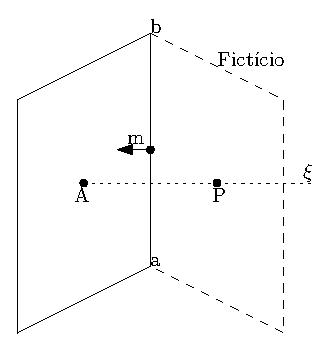
\includegraphics{fig/contorno-1.eps}
    \caption{Volume Espelhado}
    \label{contorno-1}
\end{figure}

Outro modo de se aplicar as condições de contorno com volumes fictícios é feita empregando-se um volume antissimétrico, ou seja, ele deve ser espelhado em ambas as direções (e e y), como se segue:

\subsection{Volume antissimétrico}

\begin{figure}[]
    \centering
    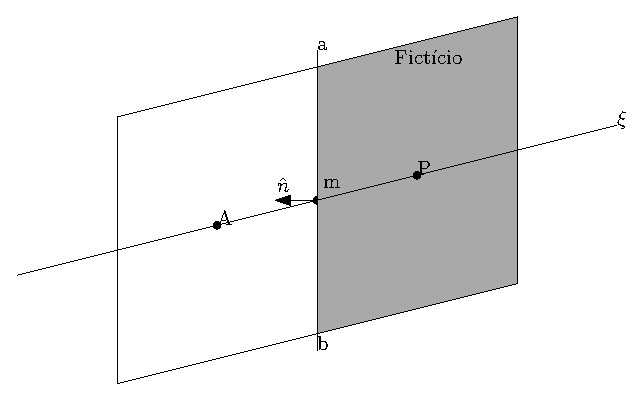
\includegraphics{fig/contorno-2.eps}
    \caption{Volume Antissimétrico}
    \label{contorno-2}
\end{figure}

Neste caso, a linha que une P e A passa pelo ponto médio da face $(m)$. Assim, não há o erro de não-ortogonalidade existente ao se aplicar o volume fictício espelhado (simétrico). Nota-se, contudo, que será necessário avaliar o termo de difusão cruzada, uma vez que o vetor normal $\hat{n}$ e o vetor unitário na direção $\xi$ podem não ser coincidentes. Nesse caso, será necessário empregar uma expressão semelhante à equação \ref{8.27}. Contudo, a temperatura nos vértices $T_a$ e $T_b$ pode ser avaliada mediante o uso das condições de contorno.

Uma importante observação a respeito da utilização de diferenças centrais envolvidas na integração da superfície dos elementos de controle diz respeito ao fato que sua acurácia será de segunda ordem apenas no caso em que as mesmas sejam avaliadas no ponto médio de $\hat{n} \cdot \vec{\nabla}T \Delta A_i$. Este não é o caso se as linhas PA e ab não se interceptam no ponto médio m de ab quando a malha é não-ortogonal.

Este erro aumenta com a não-ortogonalidade e a razão de aspecto da malha, de modo que um grande esforço deve ser feito com relação ao controle da não-ortogonalidade e da razão de aspecto em malhas não-estruturadas.
